\begin{frame}{Neural network architecture with three convolutional layers}
\begin{center}
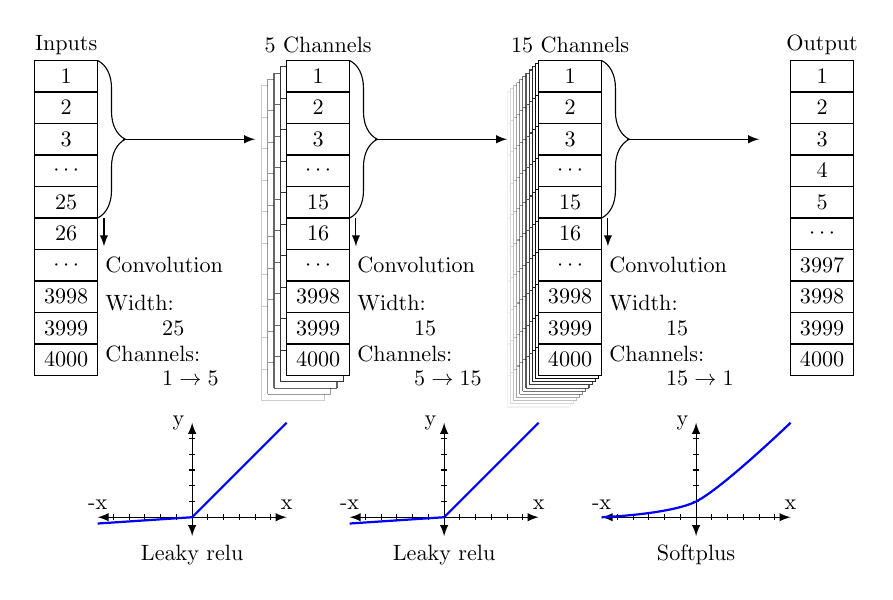
\begin{tikzpicture}[
    scale=.8,
    every node/.style={scale=.8}]
% Layer 1
\begin{scope}
\node at (0,0) {Inputs};
\foreach \i [count=\xi] in {1,2,3,$\cdots$,25,26,$\cdots$,3998,3999,4000} {
    \node at(0, -\xi/2) [draw, minimum width = 1cm, minimum height = .5cm] {\i};
}

\draw [decorate,decoration={brace,amplitude=10pt}] (.5,-.25) -- (.5,-2.75);
\draw [-latex] (.6, -2.75) -- (.6, -3.2);
\draw [-latex] (.9, -1.5) -- (3, -1.5);
\begin{scope}[xshift=.5cm, yshift=-3.5cm]
\node at (0, 0) [right] {Convolution};
\node at (0,  -.6) [right] {Width:};
\node at (.9, -1) [right] {25};
\node at (0, -1.4) [right] {Channels:};
\node at (.9, -1.8) [right] {$1\rightarrow5$};
\end{scope}
\end{scope}

% Layer 2
\begin{scope}[xshift=4cm]
\node at (0,0) {5 Channels};
% Backing
\foreach \i in {.4,.3,.2,.1} {
\begin{scope}[xshift=-.5cm-\i cm, yshift=-.25cm -\i cm]
\path[fill=white] (0,0) rectangle (1,-5);
\draw [opacity=1-\i*2, ystep=.5] (0,0) grid (1,-5);
\end{scope}
}
\foreach \i [count=\xi] in {1,2,3,$\cdots$,15,16,$\cdots$,3998,3999,4000} {
    \node at(0, -\xi/2) [draw, fill=white, minimum width = 1cm, minimum height = .5cm] {\i};
}

\draw [decorate,decoration={brace,amplitude=10pt}] (.5,-.25) -- (.5,-2.75);
\draw [-latex] (.6, -2.75) -- (.6, -3.2);
\draw [-latex] (.9, -1.5) -- (3, -1.5);
\begin{scope}[xshift=.5cm, yshift=-3.5cm]
\node at (0, 0) [right] {Convolution};
\node at (0,  -.6) [right] {Width:};
\node at (.9, -1) [right] {15};
\node at (0, -1.4) [right] {Channels:};
\node at (.9, -1.8) [right] {$5\rightarrow15$};
\end{scope}
\end{scope}

% Layer 3
\begin{scope}[xshift=8cm]
\node at (0,0) {15 Channels};
% Backing
\foreach \i in {.5,.45,.4,.35,.3,.25,.2,.15,.1,.05} {
\begin{scope}[xshift=-.5cm-\i cm, yshift=-.25cm -\i cm]
\path[fill=white] (0,0) rectangle (1,-5);
\draw [opacity=1-\i*2 + .05, ystep=.5] (0,0) grid (1,-5);
\end{scope}
}
\foreach \i [count=\xi] in {1,2,3,$\cdots$,15,16,$\cdots$,3998,3999,4000} {
    \node at(0, -\xi/2) [draw, fill=white, minimum width = 1cm, minimum height = .5cm] {\i};
}

\draw [decorate,decoration={brace,amplitude=10pt}] (.5,-.25) -- (.5,-2.75);
\draw [-latex] (.6, -2.75) -- (.6, -3.2);
\draw [-latex] (.9, -1.5) -- (3, -1.5);
\begin{scope}[xshift=.5cm, yshift=-3.5cm]
\node at (0, 0) [right] {Convolution};
\node at (0,  -.6) [right] {Width:};
\node at (.9, -1) [right] {15};
\node at (0, -1.4) [right] {Channels:};
\node at (.9, -1.8) [right] {$15\rightarrow1$};
\end{scope}
\end{scope}

% Layer 4
\begin{scope}[xshift=12cm]
\node at (0,0) {Output};
\foreach \i [count=\xi] in {1,2,3,4,5,$\cdots$,3997,3998,3999,4000} {
    \node at(0, -\xi/2) [draw, fill=white, minimum width = 1cm, minimum height = .5cm] {\i};
}
\end{scope}

% Loop as needed
\foreach \i in {2,6} {
\begin{scope}[xshift=\i cm, yshift=-7.5cm]
\draw [step=.25] (-1.4, .05) grid (1.4, -.05);
\draw [step=.25] (-.05, -.2) grid (.05, 1.4);
\draw [black, latex-latex] (-1.5, 0) node[above] {-x} -- (1.5, 0) node[above] {x};
\draw [black, latex-latex] (0, -.3)  -- (0, 1.5) node[left] {y};
\draw [thick, blue](-1.5, -.1) -- (0, 0) -- (1.5,1.5);
\node at (0, -.6) {Leaky relu};
\end{scope}
}

\begin{scope}[xshift=10cm, yshift=-7.5cm]
\draw [step=.25] (-1.4, .05) grid (1.4, -.05);
\draw [step=.25] (-.05, -.2) grid (.05, 1.4);
\draw [black, latex-latex] (-1.5, 0) node[above] {-x} -- (1.5, 0) node[above] {x};
\draw [black, latex-latex] (0, -.3)  -- (0, 1.5) node[left] {y};
\draw [thick, blue, smooth]  plot coordinates {
    (-1.5, 0)
	(0, .25)
	(1.5, 1.5)};
\node at (0, -.6) {Softplus};
\end{scope}

\end{tikzpicture}
\end{center}
\end{frame}
